\documentclass[aspectratio=169,11pt]{beamer}
\usepackage[T1]{fontenc}
\usepackage[tt=false,type1=true]{libertine}
\usepackage[libertine]{newtxmath}
\usepackage{amsmath,booktabs,array,tikz,pgfpages}
\usefonttheme{serif}
\usefonttheme{professionalfonts}
\usetikzlibrary{arrows.meta,calc,fit,positioning}
\ifdefined\PRESENTERNOTES
  \setbeameroption{show notes on second screen=right}
  \hypersetup{draft}
\else
  \setbeameroption{hide notes}
\fi
\definecolor{ink}{HTML}{152B42}
\definecolor{teal}{HTML}{087E83}
\definecolor{amber}{HTML}{B46A20}
\definecolor{plum}{HTML}{6B4788}
\definecolor{quiet}{HTML}{526473}
\setbeamercolor{normal text}{fg=ink,bg=white}
\setbeamercolor{frametitle}{fg=ink,bg=white}
\setbeamercolor{structure}{fg=teal}
\setbeamercolor{alerted text}{fg=teal}
\setbeamertemplate{navigation symbols}{}
\setbeamertemplate{footline}{\hfill\color{quiet}\insertframenumber\hspace{1em}\vspace{.6em}}
\setbeamertemplate{frametitle}{\vspace{.65em}\insertframetitle\par\vspace{.3em}\noindent\textcolor{teal}{\rule{\textwidth}{.6pt}}\par}
\setbeamerfont{frametitle}{size=\Large,series=\bfseries}
\setbeamercolor{note page}{bg=white}
\setbeamercolor{note title}{fg=ink,bg=white}
\setbeamerfont{note page}{size=\small}
\tikzset{
  flow/.style={-{Latex[length=2.5mm]},line width=1.2pt,draw=teal},
  proposed/.style={flow,draw=amber},
  stage/.style={draw=ink,line width=.8pt,rounded corners=2pt,
    minimum height=11mm,align=center,inner sep=5pt},
  stage proposed/.style={stage,draw=amber},
  diagram stage/.style={stage,minimum height=7mm,inner sep=3pt},
  diagram proposed/.style={diagram stage,draw=amber},
  small label/.style={font=\small,align=center,text=quiet},
  batch/.style={draw=ink,fill=ink!4,minimum width=1.1cm,
    minimum height=.7cm,align=center,inner sep=4pt},
  link/.style={-{Latex[length=2mm]},draw=ink,line width=.8pt},
  ref/.style={link,dashed,draw=quiet}
}
\newcommand{\source}[1]{\par\vfill{\color{quiet}\scriptsize #1}}
\newcommand{\lead}[1]{{\color{teal}\bfseries #1}}


\newcommand{\join}{\mathbin{\bowtie}}
\newcommand{\emptyrow}{\textcolor{quiet}{no rows}}



\title{DBSP Physical Design: Advisor Presentation}
\date{2026-10-08}

\begin{document}

% Preserve geometry while revealing future rows and fading completed steps.
\newcommand{\reveal}[3]{\uncover<#1->{\alt<#2>{\textcolor{teal}{#3}}{\textcolor{quiet}{#3}}}}

% 1
\begin{frame}{DBSP: incremental computation and physical state}
  \large
  Budiu et al., DBSP, VLDB 2023: Theoretical Generality\par
  \lead{Physical Design: available only from codebase.}
  \par\medskip
  E.g., how does DBSP retain, share, merge, and place \emph{intermediate states} required
  for incremental maintenance?
  \note{Timing: 1 minute. DBSP supplies a theory and implementation of incremental computation: update a maintained result from signed input changes instead of evaluating the complete query again. A weighted relation can express insertions, retractions, and multiplicities. Integration accumulates changes. Generality and composability are established theoretical context, not the focus of this talk. We recover the physical behavior from the inspected implementation: retained state, indexed representations, immutable runs, snapshots, merging, and memory controls. The Orders--Lineitem-first program is an equivalent explanatory choice. The existing experiment uses Orders--Customer first and is identified separately at the end. Theory: VLDB 2023 Sections 2.3 and 3. Physical claims: SOURCE-EVIDENCE.md.}
\end{frame}

% 2
\begin{frame}<1-2>{Storage for base relations}
  \centering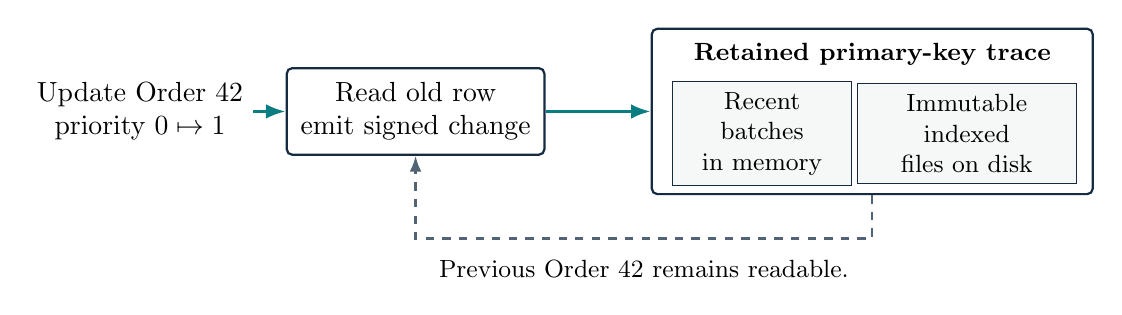
\begin{tikzpicture}[x=1cm,y=1cm,font=\normalsize]
  \node[align=center] (update) at (0,1.4) {Update Order 42\\priority $0\mapsto1$};
  \node[stage] (upsert) at (3.5,1.4) {Read old row\\emit signed change};
  \node[stage,minimum width=5.6cm,minimum height=2.1cm] (trace) at (9.3,1.4) {};
  \node[font=\small\bfseries] at (9.3,2.12) {Retained primary-key trace};
  \node[batch,font=\small,text width=2cm] (mem) at (7.9,1.12) {Recent batches\\in memory};
  \node[batch,font=\small,text width=2.5cm] (disk) at (10.5,1.12) {Immutable indexed\\files on disk};
  \draw[flow] (update.east) -- (upsert.west);
  \draw[flow] (upsert.east) -- (trace.west);
  \draw[ref] (trace.south) -- ++(0,-.55) -| (upsert.south);
  \node[font=\small] at (6.4,-.6) {Previous Order 42 remains readable.};
\end{tikzpicture}

  \source{trace/spine\_async.rs; storage/file.rs; file/indexed\_wset\_batch.rs.}
  \note{Timing: 1.5 minutes across two advances. An already-loaded static Orders table has a primary-key map interface and retains immutable indexed runs, in memory or configured file storage. Levels and run sizes are schematic, not disjoint key ranges or an exact schedule. Each run has an independent rightward cursor, visible on both advances. Runs can overlap; a trace cursor combines matching key/value contents and signed weights. Native file ``columns'' describe nested file trees, not SQL attribute columns. The key tree and value tree each have index blocks above data leaves. Untimed indexed leaf items are (K, ()) and (V, weight); values are ordered within each key's group. Sources: storage/file.rs:3--65; trace/ord/file/indexed\_wset\_batch.rs:41--83; trace/cursor/cursor\_list.rs.}
  \note<1>{\par Structure: three, two, and one immutable runs illustrate the LSM-like spine. The dashed connector enlarges one file, with an index root and two leaves per tree. Key data-block metadata supplies the next-column row range, separately from (K, ()). Index blocks hold child bounds, cumulative row totals, byte offsets, and sizes. Data blocks hold item offsets and next-column row groups. Actual scheduling uses level counts and background merge/pressure triggers. Sources: storage/file/format.rs:15--62; trace/spine\_async.rs.}
  \note<2>{\par Lookup: seek Order ID 43 independently in each retained run. In the enlarged file, descend to the matching key leaf. Its two row boundaries give [start, end). Locate the first value row, start, by cumulative row totals in the value tree; then iterate the group until end. There is no target V in this lookup. The arrow denotes row-range navigation, not a direct byte pointer to a separate per-key tree. Appendix E expands this traversal. Combine weighted matches across overlapping runs; do not assume one matching run or one physical value per key. Sources: storage/file/reader.rs; trace/cursor/cursor\_list.rs.}
\end{frame}

% 3
\begin{frame}[fragile]{Creating an immutable run}
  \small
  \textbf{Native LSM storage insufficiency:} NO mutable memtable across transactions.
  Delta from ONE transaction becomes ONE IMMUTABLE run.
  \par\smallskip
  \begin{columns}[T,onlytextwidth]
    \begin{column}{.56\textwidth}
      \fontsize{8}{8}\selectfont
\begin{verbatim}
struct Writer:
    key_tree: TreeWriter
    value_tree: TreeWriter
struct TreeWriter:
    rows = [0, 0)
    leaf_builder
    index_builders

write1(item):
    value_tree.rows.end += 1
    value_tree.append(item)

write0(item):
    r = value_tree.rows
    assert r.start < r.end
    value_tree.rows = [r.end, r.end)
    key_tree.rows.end += 1
    key_tree.append(item, row_group=r)
\end{verbatim}
    \end{column}
    \begin{column}{.42\textwidth}
      \fontsize{8}{8}\selectfont
\begin{verbatim}
// Input sorted lexicographically
// by (K, V)
for each K and its value group:
    for each (V, weight) in the group:
        writer.write1((V, weight))
    writer.write0((K, ()))
writer.close(metadata)
\end{verbatim}
      \par\bigskip\small
      \textbf{Key 43: two value writes}\par\smallskip
      Pending rows: $[2,2)\to[2,3)\to[2,4)$.\par\medskip
      \texttt{write0((43, ()))} captures $[2,4)$\par
      and resets pending rows to $[4,4)$.
    \end{column}
  \end{columns}
  \note{Timing: 1.5 minutes. The callout describes the illustrated one-run case in the inspected input/join paths: there is no mutable memtable absorbing updates across transactions. An actual transaction can produce several runs. This simplified file writer constructs one immutable run across many write1 and write0 calls, completing it at close(metadata), not at each individual write. Native file ``columns'' mean nested file trees, not SQL attribute columns: key\_tree and value\_tree replace that terminology here. TreeWriter stands for ColumnWriter; leaf\_builder and index\_builders stand for its data\_block and index\_blocks. Serialization, factories, errors, buffering, and trailer details are omitted. Input has distinct sorted keys and nonempty value groups with distinct sorted values after consolidation. Row ordinals are file-wide within each tree, not leaf-local. A leaf flush does not reset the tree's counters. write1 has no position argument: it increments value\_tree.rows.end and appends the item. write0 takes the pending nonempty value-row range, resets it to [end,end), increments the key-tree counter, and appends (K, ()) with that row group. For key 43, two writes move pending rows from [2,2) through [2,3) to [2,4); the key write captures [2,4) and resets to [4,4). Sources: storage/file/writer.rs:224--246,1234--1255,1660--1737.}
\end{frame}

% 4
\begin{frame}{Ex. predicate-free three-way join}
  \begin{columns}[T,onlytextwidth]
    \begin{column}{.53\textwidth}
      $V=\text{Customer}\join\text{Orders}\join\text{Lineitem}$\par
      Notations:\par
      $R^-$ \quad $R^+$ \quad $\Delta R=R^+-R^-$
    \end{column}
    \begin{column}{.44\textwidth}
      \textbf{Before the transaction}\par\smallskip
      \small
      \begin{tabular}{ll}
        \toprule Customer & Segment\\\midrule
        7 & BUILDING\\\bottomrule
      \end{tabular}\par\smallskip
      \begin{tabular}{ll}
        \toprule Order & Customer\\\midrule
        42 & 7\\\bottomrule
      \end{tabular}\par\smallskip
      \begin{tabular}{lll}
        \toprule Order & Line & Price\\\midrule
        42 & 1 & 100\\\bottomrule
      \end{tabular}
    \end{column}
  \end{columns}
  \par\smallskip
  \note{Timing: 1.5 minutes. This SQL projection is the experiment's maintained view, not full TPC-H Q3. It has two equijoins and retains all nine projected fields. There are no Q3 filters, aggregate, ranking, or limit here. Customer 7 has segment BUILDING. Order 42 has customer 7, date 1995-03-01, and ship priority 0. Its line 1 has price 100, discount 0, and ship date 1995-03-10. Primary keys are Customer ID, Order ID, and (Order ID, line number). We will insert Order 43, dated 1995-03-02 with priority 0, and its line 1, priced 30 with discount 0 and ship date 1995-03-11, in the same transaction. The tables show the identifying fields. Appendix A defines complete payloads. The chosen explanatory join order changes no SQL result. R superscript minus and plus name states, not negative and positive row weights. Source: experiments/q3-ivm-baseline/query.sql:1--30.}
\end{frame}

% 5
\begin{frame}{The complete incremental program}
  \resizebox{.98\textwidth}{!}{%
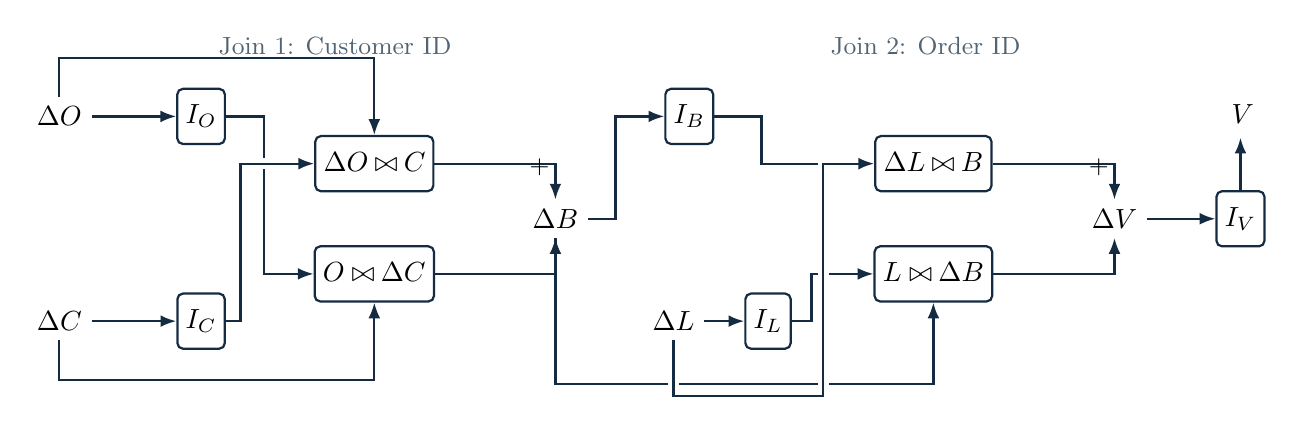
\begin{tikzpicture}[x=1cm,y=1cm,font=\normalsize]
  % Two branches per join. Small I boxes name every retained input.
  \node (do) at (0,3.4) {$\Delta O$};
  \node (dc) at (0,.8) {$\Delta C$};
  \node[diagram stage] (ic) at (1.8,.8) {$I_C$};
  \node[diagram stage] (io) at (1.8,3.4) {$I_O$};
  \node[diagram stage] (j1a) at (4.0,2.8) {$\Delta O\join C_{\current}$};
  \node[diagram stage] (j1b) at (4.0,1.4) {$O_{\before}\join\Delta C$};
  \node (db) at (6.3,2.1) {$\Delta B$};
  \draw[link] (do) -- (io);
  \draw[link] (dc) -- (ic);
  \draw[link] (do.north) -- ++(0,.5) -| (j1a.north);
  \draw[link] (dc.south) -- ++(0,-.5) -| (j1b.south);
  \draw[link] (io.east) -- (2.6,3.4) |- (j1b.west);
  \draw[link,preaction={draw=white,line width=4pt,-}]
    (ic.east) -- (2.3,.8) |- (j1a.west);
  \draw[link] (j1a.east) -| (db.north);
  \draw[link] (j1b.east) -| (db.south);
  \node[font=\small] at (6.1,2.75) {$+$};
  \node[diagram stage] (ib) at (8.0,3.4) {$I_B$};
  \node (dl) at (7.8,.8) {$\Delta L$};
  \node[diagram stage] (il) at (9.0,.8) {$I_L$};
  \node[diagram stage] (j2a) at (11.1,2.8) {$\Delta L\join B_{\current}$};
  \node[diagram stage] (j2b) at (11.1,1.4) {$L_{\before}\join\Delta B$};
  \node (dv) at (13.4,2.1) {$\Delta V$};
  \node[diagram stage] (iv) at (15,2.1) {$I_V$};
  \node (v) at (15,3.4) {$V_{\current}$};
  \draw[link] (db.east) -- ++(.35,0) |- (ib.west);
  \draw[link] (ib.east) -- ++(.6,0) |- (j2a.west);
  \draw[link] (dl.east) -- (il.west);
  \draw[link] (il.east) -- ++(.25,0) |- (j2b.west);
  \draw[link] (db.south) -- ++(0,-1.85) -| (j2b.south);
  \draw[link,preaction={draw=white,line width=4pt,-}]
    (dl.south) -- (7.8,-.15) -- (9.7,-.15) -- (9.7,2.8) -- (j2a.west);
  \draw[link] (j2a.east) -| (dv.north);
  \draw[link] (j2b.east) -| (dv.south);
  \node[font=\small] at (13.2,2.75) {$+$};
  \draw[link] (dv.east) -- (iv.west);
  \draw[link] (iv.north) -- (v.south);
  \node[font=\small,text=quiet] at (3.5,4.3) {Join 1: Customer ID};
  \node[font=\small,text=quiet] at (11,4.3) {Join 2: Order ID};
\end{tikzpicture}}

  \vspace{-1em}
  \begin{align*}
    \Delta OL &= \Delta L\join O^+ + L^-\join\Delta O\\
    \uncover<2->{\Delta V} &\uncover<2->{= \Delta OL\join C^+ + OL^-\join\Delta C}
  \end{align*}
  \par\raggedright
  $\mathcal{I}_{\Delta R}$ ``integrates'' $\Delta R$
\end{frame}

% 6
\begin{frame}{Accumulated state and immutable runs}
  \begin{columns}[T,onlytextwidth]
    \begin{column}{.48\textwidth}
      \small
      \begin{tabular}{@{}ll}
        \toprule State/``Trace'' & Access key\\\midrule
        $O_o$ & Order ID\\
        $L_o$ & Order ID\\
        $OL_{c,o}$ & Customer ID\\
        $C_c$ & Customer ID\\\bottomrule
      \end{tabular}
      \smallskip\par
      Created by ``integrating'' or accumulating all deltas in the history.
    \end{column}
    \begin{column}{.49\textwidth}
      \lead{$R^+$ and $R^-$ share one trace.}\par
    \end{column}
  \end{columns}
\end{frame}

% 7
\begin{frame}{Record structure}
  \large Logically, $\text{record}=(\text{key},\text{value},\text{weight})$---``bag semantics''
  \par\medskip\normalsize
  Physically, $OL_{c,o}$ is stored as
  \begin{center}\small
    \begin{tabular}{@{}lll@{}}
      % Pending physical layout
      % \toprule Key & Value & Weight\\\midrule
      % 7 & $(42,1,\text{1995-03-01},0,100,0,\text{1995-03-10})$ & $+1$\\
      % 7 & $(43,1,\text{1995-03-02},0,30,0,\text{1995-03-11})$ & $+1$\\\bottomrule
    \end{tabular}
  \end{center}
  \par\medskip
  \begin{columns}[T,onlytextwidth]
    \begin{column}{.46\textwidth}
      \textbf{Multiplicity}\par
      $+2$: two equal complete rows.\par
      A join multiplies matching weights.
    \end{column}
    \begin{column}{.49\textwidth}
      \textbf{Signed transaction delta}\par
      $-1$: retract one row.\par
      Equal pairs cancel: $+1+(-1)=0$.
    \end{column}
  \end{columns}
  \source{Weighted relations: VLDB 2023 \S4. Indexed/nested groups: \S7.3.}
  \note{Timing: 1 minute. The native indexed run key is Customer ID. The subscript c,o describes grouping and value ordering, not a composite native key: Order ID then line number lead the value tuple. A row is identified explicitly, for example (7;43,1,...). Remaining value fields are Order date, priority, line price, discount, ship date. No segment is present until the Customer join. Distinct complete values share key 7. Equal complete key/value pairs consolidate into integer multiplicities; zero totals disappear. Neither weight nor visibility superscript is a record identity or transaction timestamp. The underlying representation supports weighted bags even when source primary-key map semantics impose uniqueness. Sources: VLDB 2023 Sections 4 and 7.3; indexed\_wset\_batch.rs.}
\end{frame}

% 8
\begin{frame}{Memory arrays and indexed file groups}
  \small
  One illustrative $OL_{c,o}$ run. Arrays preserve complete values and weights.
  \par\medskip
  \begin{tabular}{@{}ll@{}}
    Keys & $[7,9]$\\[.3em]
    Group offsets & $[0,2,3]$\\[.3em]
    Values & $[(42,1,\text{1995-03-01},0,100,0,\text{1995-03-10}),$\\
      & $\phantom{[}(43,1,\text{1995-03-02},0,30,0,\text{1995-03-11}),$\\
      & $\phantom{[}(44,1,\text{1995-03-03},0,50,0,\text{1995-03-12})]$\\[.3em]
    Weights & $[1,1,1]$\\
  \end{tabular}
  \par\smallskip\centering
  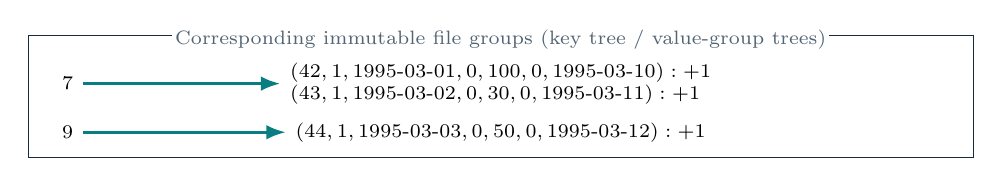
\begin{tikzpicture}[x=1cm,y=.65cm,font=\scriptsize]
  \node[draw=ink,minimum width=12cm,minimum height=1.55cm] at (6,0) {};
  \node[text=quiet,fill=white,inner sep=1pt] at (6,1.1) {Corresponding immutable file groups (key tree / value-group trees)};
  \node (k7) at (.5,.25) {$7$};
  \node[align=left] (v7) at (6,.25) {$(42,1,\text{1995-03-01},0,100,0,\text{1995-03-10}):+1$\\
    $(43,1,\text{1995-03-02},0,30,0,\text{1995-03-11}):+1$};
  \node (k9) at (.5,-.7) {$9$};
  \node (v9) at (6,-.7) {$(44,1,\text{1995-03-03},0,50,0,\text{1995-03-12}):+1$};
  \draw[flow] (k7.east) -- (v7.west);
  \draw[flow] (k9.east) -- (v9.west);
\end{tikzpicture}

  \par\smallskip\raggedright
  Key 7 selects values $[0,2)$; key 9 selects $[2,3)$.\par
  Compatible memory/file cursors seek keys and iterate values and weights.
  \source{VecIndexedWSet::from\_parts; storage/file.rs. Customer 9 / Order 44 is a layout-only extension.}
  \note{Timing: 1.5 minutes. The sorted key array and half-open group offsets identify contiguous value ranges. Each value carries the full OL payload. The immutable layer file contains the same concrete key/value groups, with tree indexes within the file. The diagram is a logical grouping, not a byte-level layout. The spine organizes runs separately from indexes within a file. A trace may retain both memory and file runs and expose compatible cursors. Extra Customer 9 and Order 44/line 1, price 50 and ship date 1995-03-12, illustrate a second group only. They do not change the running transaction. Sources: trace/ord/vec/indexed\_wset\_batch.rs:158--199; storage/file.rs:3--65.}
\end{frame}

% 9
\begin{frame}{A changed Customer reads retained intermediate rows}
  \centering\resizebox{.95\textwidth}{!}{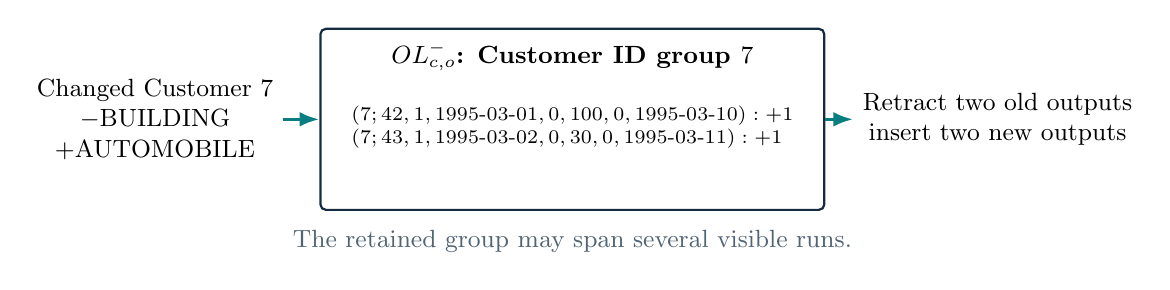
\begin{tikzpicture}[x=1cm,y=1cm,font=\small]
  \node[align=center] (delta) at (0,1.3) {Changed Customer 7\\$-\text{BUILDING}$\\$+\text{AUTOMOBILE}$};
  \node[stage,minimum width=6.4cm,minimum height=2.3cm] (group) at (5.3,1.3) {};
  \node[font=\small\bfseries] at (5.3,2.1) {$OL_{c,o}^-$: Customer ID group $7$};
  \node[font=\scriptsize,align=left] at (5.3,1.2) {$(7;42,1,\text{1995-03-01},0,100,0,\text{1995-03-10}):+1$\\
    $(7;43,1,\text{1995-03-02},0,30,0,\text{1995-03-11}):+1$};
  \node[align=center] (out) at (10.7,1.3) {Retract two old outputs\\insert two new outputs};
  \draw[flow] (delta.east) -- (group.west);
  \draw[flow] (group.east) -- (out.west);
  \node[font=\small,text=quiet] at (5.3,-.25) {The retained group may span several visible runs.};
\end{tikzpicture}
}
  \par\medskip\raggedright
  Customer 7 changes BUILDING to AUTOMOBILE. $OL_{c,o}$ stays unchanged.
  \par\smallskip\small
  For each retained row $r=(7;o,1,\ldots)$, where $o\in\{42,43\}$:\par
  $-(7,\text{BUILDING},o,\text{date},0,1,\text{price},0,\text{shipdate})$\par
  $+(7,\text{AUTOMOBILE},o,\text{date},0,1,\text{price},0,\text{shipdate})$
  \par\smallskip\normalsize
  Consolidate matching values across visible runs, then project signed outputs.
  \source{Logical match on Customer ID. Cursor seeks/value iteration: trace/cursor.rs. Full payloads: Appendix A.}
  \note{Timing: 1.5 minutes. This occurs after the insertion transaction. Customer overwrite emits negative (7,BUILDING) and positive (7,AUTOMOBILE). The first Orders--Lineitem join has no changed inputs, so delta OL is empty and OL remains unchanged. The second join's Customer-change branch reads OL before-state directly and finds both retained lines for Orders 42 and 43. Their dates/prices/ship dates are respectively 1995-03-01/100/1995-03-10 and 1995-03-02/30/1995-03-11. Priority and discount are zero. Each yields a negative old nine-field output and positive new output, changing only the segment. Matching values may span several runs. Trace cursors consolidate complete key/value weights across those runs. The example shows logical matches, not a mandatory delta-led scan. Optional fetch\_join prepares requested keys and is configuration-gated; ordinary joins can choose driving direction by estimated key counts. Sources: join.rs:705--749,1760--1788; trace/cursor.rs; cursor/cursor\_list.rs.}
\end{frame}

% 10
\begin{frame}{Small updates become separate immutable runs}
  \lead{Native storage shortcoming: no mutable memtable across transactions}
  \par\smallskip\small
  in the inspected input and join paths. Each output seals before trace insertion.
  \par\medskip\centering
  \resizebox{.98\textwidth}{!}{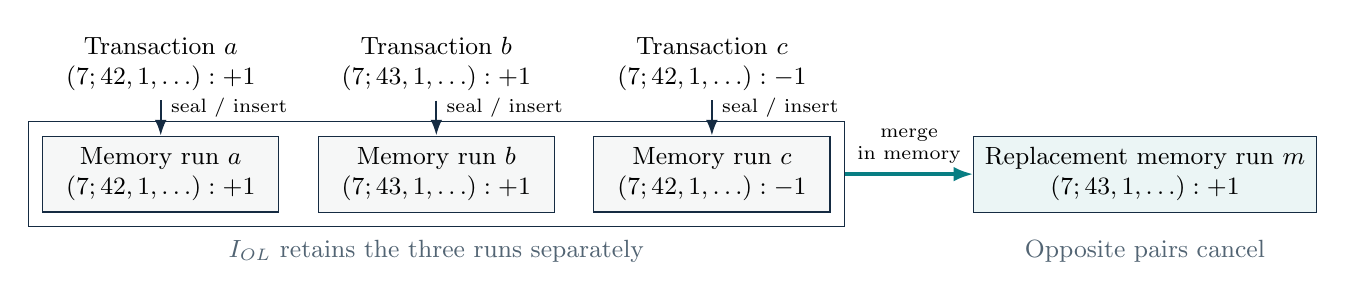
\begin{tikzpicture}[x=1cm,y=.7cm,font=\small]
  \foreach \x/\id/\change in {0/a/{(7;42,1,\ldots):+1},3.5/b/{(7;43,1,\ldots):+1},7/c/{(7;42,1,\ldots):-1}} {
    \node[align=center] (d\id) at (\x,3.5) {Transaction $\id$\\$\change$};
    \node[batch,minimum width=3cm] (r\id) at (\x,1.5) {Memory run $\id$\\$\change$};
    \draw[link] (d\id) -- node[pos=.2,right,font=\scriptsize] {seal / insert} (r\id);
  }
  \node[draw=ink,fit=(ra)(rb)(rc),inner sep=5pt] (trace) {};
  \node[font=\small,text=quiet] at (3.5,.1) {$I_{OL}$ retains the three runs separately};
  \node[batch,fill=teal!8,minimum width=3cm] (m) at (12.5,1.5) {Replacement memory run $m$\\$(7;43,1,\ldots):+1$};
  \draw[flow] (trace.east) -- node[above,align=center,font=\scriptsize] {merge\\in memory} (m.west);
  \node[font=\small,text=quiet] at (12.5,.1) {Opposite pairs cancel};
\end{tikzpicture}
}
  \par\medskip\raggedright\normalsize
  Larger runs grow through merging, including \textbf{merging in memory}.\par\smallskip
  One transaction can produce several runs. A merged run can combine several\par
  transactions, and cancellation can remove their contributions.\par\smallskip
  There is no fixed number of transactions per run.
  \source{Illustrative run sizes and merge timing. Structural limitation; performance consequences are unmeasured.}
  \note{Timing: 1.5 minutes. The OL example shows one-record memory runs: a inserts (7;42,1,...), b inserts (7;43,1,...), c retracts the first pair. Each seals before separate trace insertion. There is no mutable memtable across transactions in these paths. A later memory merge constructs a replacement; cancellation leaves only the second pair. Run sizes and merge timing are illustrative. Native scheduling uses levels/counts and pressure/compaction triggers, not this exact three-run schedule. Merging can also choose file output. One transaction may yield several runs; merged runs may combine several transactions. Neither size nor transaction count is fixed. The default 10,000-record join-output chunk target can overshoot when buffered output is submitted and seals final partial output. It does not cap input-map or merged runs. Placement thresholds choose where runs live. Root-circuit untimed runs carry no per-record transaction epoch; timed batches exist elsewhere. Performance consequences remain unmeasured. Sources: input\_upsert.rs:691; input\_upsert.rs:321; join.rs:1926--1957; dev\_tweaks.rs:332; spine\_async.rs:310--365,446--463; fallback/indexed\_wset.rs:546--560.}
\end{frame}

% 11
\begin{frame}{Before-state and after-state snapshots}
  \centering% Each snapshot holds one reference per run; runs stack by level, the new one joins the top level.
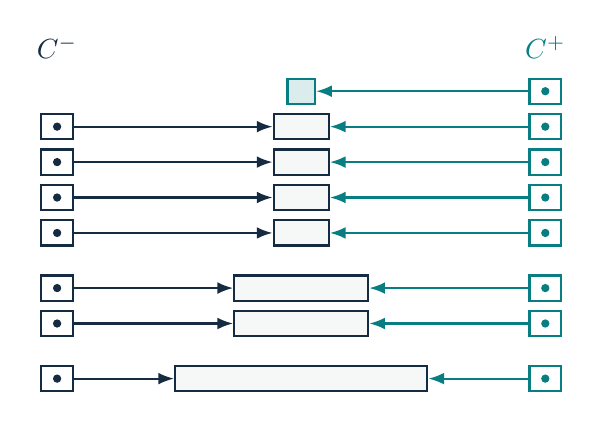
\begin{tikzpicture}[x=1cm,y=1cm,font=\normalsize,
  run/.style={draw=ink,fill=ink!4,line width=.8pt,minimum height=.32cm,
    inner sep=0pt},
  slot/.style={draw=#1,line width=.8pt,minimum width=.4cm,minimum height=.32cm,
    inner sep=0pt},
  pointer/.style={-{Latex[length=2mm]},draw=#1,line width=.8pt}]
  % Levels: small runs plus the new transaction's smaller run, then medium and large.
  \node[run,fill=teal!15,draw=teal,minimum width=.35cm] (run0) at (4,4.05) {};
  \foreach \i/\y/\w in {1/3.6/.7,2/3.15/.7,3/2.7/.7,4/2.25/.7,
                        5/1.55/1.7,6/1.1/1.7,7/.4/3.2}
    \node[run,minimum width=\w cm] (run\i) at (4,\y) {};

  % Before-state references every retained run; after-state also the new one.
  \node[text=ink] at (.9,4.6) {$C^-$};
  \node[text=teal] at (7.1,4.6) {$C^+$};
  \foreach \i in {1,...,7} {
    \node[slot=ink] (before\i) at (run\i -| .9,0) {};
    \fill[ink] (before\i) circle (1.5pt);
    \draw[pointer=ink] (before\i) -- (run\i.west);
  }
  \foreach \i in {0,...,7} {
    \node[slot=teal] (after\i) at (run\i -| 7.1,0) {};
    \fill[teal] (after\i) circle (1.5pt);
    \draw[pointer=teal] (after\i) -- (run\i.east);
  }
\end{tikzpicture}

  \par\bigskip
  \large
  A snapshot copies references to complete immutable runs.\par\medskip\normalsize
  $OL_{c,o}^-$ and $OL_{c,o}^+$ share unchanged runs.\par\smallskip
  After-state includes the new run. Before-state excludes it.
  \source{Snapshot strong references: trace/spine\_async/snapshot.rs:55--63,170--179.}
  \note{Timing: 1 minute. Return to the transaction inserting Order 43 and its line. Before-state OL references run a for Order 42/line 1. After-state references the same a plus newly inserted run b for Order 43/line 1. Snapshot creation clones strong references, not records. This is illustrative membership: actual transactions may supply several runs, and merged runs may combine contributions from several transactions. Superscripts identify visibility, not signed tuple weights or a homogeneous epoch for all records in a run. A delayed trace accessor selects before-state without another independent integrator. Sources: snapshot.rs:55--63,170--179; accumulate\_trace.rs delayed accessor and flush snapshot.}
\end{frame}

% 12
\begin{frame}{Merging referenced runs}
  \centering\resizebox{.95\textwidth}{!}{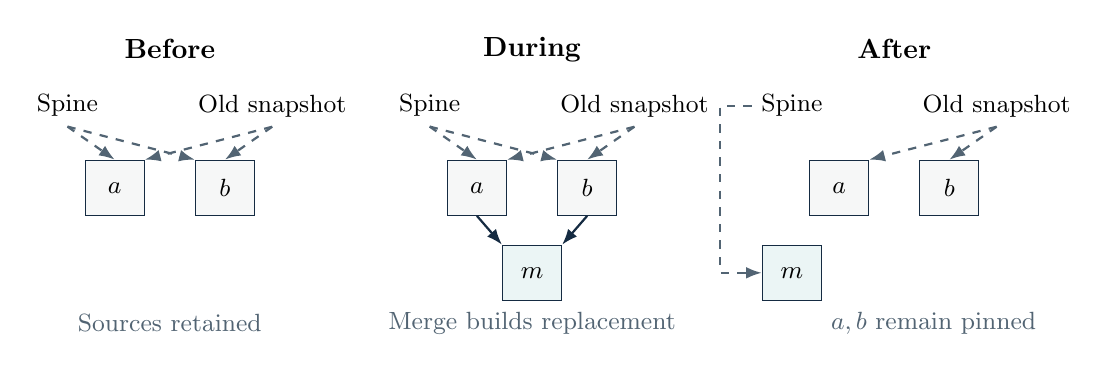
\begin{tikzpicture}[x=1cm,y=.8cm,font=\small]
  \foreach \x/\id/\label in {0/one/Before,4.6/two/During,9.2/three/After} {
    \node[font=\normalsize\bfseries] at (\x+1.3,3.4) {\label};
    \node (s\id) at (\x,2.5) {Spine};
    \node (r\id) at (\x+2.6,2.5) {Old snapshot};
    \node[batch,minimum width=.75cm] (a\id) at (\x+.6,1.2) {$a$};
    \node[batch,minimum width=.75cm] (b\id) at (\x+2,1.2) {$b$};
    \draw[ref] (r\id.south) -- (a\id.north east);
    \draw[ref] (r\id.south) -- (b\id.north);
  }
  \draw[ref] (sone.south) -- (aone.north);
  \draw[ref] (sone.south) -- (bone.north west);
  \draw[ref] (stwo.south) -- (atwo.north);
  \draw[ref] (stwo.south) -- (btwo.north west);
  \node[batch,fill=teal!8,minimum width=.75cm] (m4) at (5.9,-.15) {$m$};
  \draw[link] (atwo.south) -- (m4.north west);
  \draw[link] (btwo.south) -- (m4.north east);
  \node[font=\small,text=quiet] at (5.9,-.95) {Merge builds replacement};
  \node[batch,fill=teal!8,minimum width=.75cm] (m9) at (9.2,-.15) {$m$};
  \draw[ref] (sthree.west) -- ++(-.4,0) |- (m9.west);
  \node[font=\small,text=quiet] at (11,-.95) {$a,b$ remain pinned};
  \node[font=\small,text=quiet] at (1.3,-.95) {Sources retained};
\end{tikzpicture}
}
  \par\medskip
  \lead{Merge completion releases the spine's source references.}\par\smallskip
  An old snapshot can still own the old runs.\par\medskip
  Reclaim a memory run after its last strong owner releases it.
  \source{Snapshot Arcs, merge slots, and merge\_complete: snapshot.rs and spine\_async.rs.}
  \note{Timing: 1.5 minutes. Before the merge, the spine and old snapshot own a and b. During the merge, the merge machinery retains the inputs while building m, so source data and replacement data coexist. At completion the spine installs m and releases its source references. The snapshot still owns a and b until its consumers finish, so completion alone cannot reclaim their memory. The exact lifetime is the final strong owning reference, including any other readers. Spilling shared memory similarly writes a file-backed copy while readers retain the original. For newly created temporary file runs, reader ownership keeps the underlying file alive and DeleteOnDrop removes it when the last owner drops. Checkpoint-marked or reopened persistent files have different keep/delete behavior. That qualification is about retention, not a recovery-design claim. Sources: snapshot.rs:55--63; spine\_async.rs:527--575, 2457--2504; posixio\_impl.rs:615--635.}
\end{frame}

% 13
\begin{frame}{Where memory goes}
  \begin{tabular}{@{}p{.24\textwidth}p{.71\textwidth}@{}}
    \toprule Allocation & Examples\\\midrule
    Retained state & Base-input state, join traces, materialized $V$\\[.8em]
    Temporary or pinned & Transaction runs, merge output under construction, obsolete runs held by snapshots\\[.8em]
    Cache and lookup & Storage block cache, resident filters, index metadata\\[.8em]
    Other allocations & Connector buffers, stacks, allocator overhead, other work\\\bottomrule
  \end{tabular}
  \par\bigskip
  \large\lead{Process RSS measures resident memory across these allocations.}\par\medskip\normalsize
  Count shared allocations once. File bytes do not equal resident bytes.
  \source{runtime.rs RSS sampling; operator/run metrics; buffer\_cache/cache.rs; operations/memory.md.}
  \note{Timing: 1.5 minutes. Memory accounting must include primary-key input traces as well as join and output state. During maintenance there are transaction runs, exchange or other in-flight runs, merge-building allocations, and old sources pinned by snapshots. Disk state still needs a memory cache and resident lookup filters/metadata. The process also contains connector buffers, thread stacks, allocator overhead, and other allocations. Operator allocation estimates, run and merge metrics, cache occupancy, and filter memory are useful diagnostics, but they are not interchangeable with process RSS. Summing per-operator estimates blindly can count shared runs more than once. The on-disk file size is not its resident memory footprint. This slide classifies native allocations and makes no measured per-state or savings claim. Sources: circuit/runtime.rs:848--904; storage/buffer\_cache/cache.rs; docs.feldera.com/docs/operations/memory.md.}
\end{frame}

% 14
\begin{frame}{What memory pressure changes}
  \small
  \begin{tabular}{@{}lp{.75\textwidth}@{}}
    \toprule Raw RSS / target & Response with storage configured\\\midrule
    $<85\%$ & Inserted runs normally remain in memory. Merge output uses the configured size threshold.\\[.65em]
    $\geq85\%$ & Merge outputs target storage. Large inserted runs spill.\\[.65em]
    $\geq90\%$ & All nonempty inserted runs target storage. Loose memory runs can trigger earlier merges.\\[.65em]
    $\geq95\%$ & Transient per-step runs also target storage.\\\bottomrule
  \end{tabular}
  \par\medskip\normalsize
  RSS sampling: about once per second, with hysteresis.\par\smallskip
  Separate backpressure pauses insertion at \textbf{128 loose runs}.\par\medskip
  \lead{Spilling may copy shared data. Readers can delay reclamation.}
  \source{runtime.rs:675--694, 848--904, 1269--1356; spine\_async.rs. RSS target is not an allocator quota.}
  \note{Timing: 2 minutes. The target is runtime max\_rss\_bytes. Raw pressure is Low below 85 percent, Moderate at 85, High at 90, and Critical at 95. Actions use effective pressure with hysteresis: High persists until raw pressure becomes Low, and Critical persists until raw pressure becomes Moderate or Low. At Moderate, the inserted-run threshold is configured min\_storage\_bytes, or the default 10 MiB. At High the threshold is zero, and loose memory runs may cause merges below usual run-count thresholds. At Critical, transient nonempty step runs also target storage. The controller samples roughly once per second, so it is not a strict allocator quota or an instantaneous cap. The 128-loose-run limit controls merger backlog separately and excludes in-progress merging runs. Shared-memory spill writes a copy and may leave the original pinned. This pressure path does not resize the storage cache. Sources: runtime.rs:675--694, 848--904, 1269--1356; spine\_async.rs:455--463,680--691,882--908, 2457--2504.}
\end{frame}

% 15
\begin{frame}{Native mechanisms and reconstruction prototype}
  \begin{tabular}{@{}p{.20\textwidth}p{.74\textwidth}@{}}
    \toprule Status & State and reads\\\midrule
    \textbf{Native} & Indexed traces retain immutable runs. Joins read accumulated state with the required visibility.\\[.8em]
    \textbf{Prototype} & The restricted RF1/RF2 path reconstructs requested ranges into temporary native runs from one COL index.\\[.8em]
    \textcolor{amber}{\textbf{Deferred}} & Broader updates, direct reconstructed cursors, and comparative memory/performance results.\\\bottomrule
  \end{tabular}
  \par\medskip
  \lead{The existing prototype uses Orders--Customer first, then Lineitem.}\par\smallskip
  Actual reads: $C_c^+,O_c^-,B_o^+,L_o^-$ (Appendix D).\par\smallskip
  Subsequent RF1 inserts / RF2 deletes require referential integrity.\par
  Base primary-key state and $V$ remain separately retained.
  \source{Explanatory program: slide 5. Actual circuit: CIRCUIT.md and native-state-read-contracts.md.}
  \note{Timing: 1.5 minutes. The actual experiment joins Orders--Customer first, then Lineitem with B. Its reconstructed accesses are C after-state and O before-state keyed by Customer ID, B after-state and L before-state keyed by Order ID. It does not retain our explanatory OL-first intermediate. Reconstruction decodes/copies and may sort requested ranges into temporary native runs. Base primary-key state and materialized V stay native; the manual COL owner runs outside the Q3 graph. Supported work is subsequent complete Order/Lineitem RF1 insertion and RF2 deletion under referential integrity after setup. Customer updates, replacements, key moves, orphans, and independent Lineitem updates are excluded. General native signed examples do not expand prototype support. Direct cursors and broader updates remain deferred. The measurement qualification campaign is pending; this deck claims no measured savings, update costs, or comparative performance. Sources: experiment README; WORKFLOW.md; native-state-read-contracts.md:373--409; CIRCUIT.md:140.}
\end{frame}

\pdfstringdefDisableCommands{\def\translate#1{#1}}
\appendix
\setbeamertemplate{footline}{\hfill\color{quiet}Appendix\hspace{1em}\vspace{.6em}}

\begin{frame}{Appendix A: complete example payloads}
  \small
  \begin{tabular}{@{}ll@{}}
    \toprule Relation & Full row / indexed pair (weights $+1$)\\\midrule
    $C_c$ & $(7,\text{BUILDING})$\\[.3em]
    $O_o$ & $(42,7,\text{1995-03-01},0)$\\
     & $(43,7,\text{1995-03-02},0)$\\[.3em]
    $L_o$ & $(42,1,100,0,\text{1995-03-10})$\\
     & $(43,1,30,0,\text{1995-03-11})$\\[.3em]
    $OL_{c,o}$ & $(7;42,1,\text{1995-03-01},0,100,0,\text{1995-03-10})$\\
     & $(7;43,1,\text{1995-03-02},0,30,0,\text{1995-03-11})$\\[.3em]
    $V$ & $(7,\text{BUILDING},42,\text{1995-03-01},0,1,100,0,\text{1995-03-10})$\\
     & $(7,\text{BUILDING},43,\text{1995-03-02},0,1,30,0,\text{1995-03-11})$\\\bottomrule
  \end{tabular}
  \par\medskip\normalsize
  Subscripts name access ordering. Explicit fields identify individual rows.\par
  $OL_{c,o}$ uses Customer ID as key. Order ID and line number lead its value.
  \source{Schema and output field order: query.sql. Semicolon separates indexed key and value.}
  \note{O fields are Order ID, Customer ID, Order date, priority. L fields are Order ID, line number, price, discount, ship date. OL is our explanatory intermediate with Customer ID key and seven value fields, starting with Order ID and line number. It excludes Customer segment until the second join. V retains the nine SQL projection fields. Decimal values omit trailing zeros for readability. The representation slide's Customer 9 and Order 44/line 1 (date 1995-03-03, priority 0, price 50, discount 0, ship date 1995-03-12) are a layout-only extension. Actual experiment B is different and defined in Appendix D.}
\end{frame}

\begin{frame}{Appendix B: overwrite and simultaneous deletion}
  \small
  \textbf{Overwrite Customer 7 after Order 43's insertion.}\par
  $\Delta C_c=\{(7,\text{BUILDING}):-1,(7,\text{AUTOMOBILE}):+1\}$\par
  $\Delta OL_{c,o}=0$. Retained $OL_{c,o}$ remains unchanged.
  \par\smallskip
  \begin{tabular}{@{}p{.24\textwidth}p{.32\textwidth}p{.379\textwidth}@{}}
    \toprule Changed rows & Matching accumulated rows & Signed output\\\midrule
    $\Delta OL_{c,o}$: none & no request to $C_c^+$ & none\\
    $\Delta C_c$: $-\text{old},+\text{new}$ & $OL_{c,o}^-$: $(7;42,1,\ldots)$ & $(7,\text{BUILDING},42,\ldots):-1$\newline $(7,\text{AUTOMOBILE},42,\ldots):+1$\\
      & $OL_{c,o}^-$: $(7;43,1,\ldots)$ & $(7,\text{BUILDING},43,\ldots):-1$\newline $(7,\text{AUTOMOBILE},43,\ldots):+1$\\\bottomrule
  \end{tabular}
  \par\smallskip
  All other output fields remain as in Appendix A.
  \par\medskip
  \textbf{Then delete Order 43 and Lineitem (43,1) together.}\par
  $\Delta L_o\join O_o^+=0$; $L_o^-\join\Delta O_o=\{(7;43,1,\ldots):-1\}$.\par
  $(7,\text{AUTOMOBILE},43,\text{1995-03-02},0,1,30,0,\text{1995-03-11}):-1$.
  \source{Native signed semantics. These Customer overwrites exceed the RF1/RF2 prototype scope.}
  \note{Customer overwrite leaves OL unchanged and reads its retained rows directly in the Customer-change branch. Each complete output retracts BUILDING and inserts AUTOMOBILE, preserving all other payloads. Subsequent simultaneous deletion first checks negative Lineitem against after-state Orders: Order 43 is gone, so no output. Before-state Lineitem matches negative Order 43 and produces one negative OL pair. That pair matches current AUTOMOBILE Customer 7 and retracts the AUTOMOBILE output exactly once. Customer deletion alone would also leave OL unchanged and retract both outputs through OL before-state joined with negative Customer. Order priority overwrite emits negative old/positive new OL values; Lineitem price overwrite does likewise. The checker asserts all exact branches, multiplicities, and cancellation.}
\end{frame}

\begin{frame}{Appendix C: sources and scope}
  \begin{itemize}
    \item \href{https://docs.feldera.com/vldb23.pdf}{Budiu et al., DBSP, VLDB 2023}: integration \S2.3, incremental joins Theorem 3.4, weighted relations \S4, indexed groups \S7.3.
    \item Native implementation: input upsert, dynamic join, memory/file indexed runs, spine snapshots, merge lifecycle, RSS controller.
    \item Current experiment: \texttt{query.sql}, native state-read contracts, \texttt{CIRCUIT.md}, experiment README, workflow.
    \item \href{https://docs.feldera.com/operations/memory/}{Feldera memory documentation}: resident state, cache, lookup metadata, and process allocations.
  \end{itemize}
  \par\medskip
  \small Detailed paths, source hashes, configuration, and provenance:\par
  \texttt{SOURCE-EVIDENCE.md} alongside the editable deck.
  \source{Illustrations are schematic. No measurements, performance gains, or recovery guarantees are implied.}
  \note{Native physical behavior here assumes storage configuration and ordinary non-adaptive joins. Optional fetch changes how keys are prepared for lookup. It does not change the logical state-read contracts of the actual experiment. Storage placement determines where state resides. Checkpoint and recovery design determine what survives a failure. These are separate properties. The source evidence record identifies the inspected implementation and its configuration. The existing RF1/RF2 prototype supports only the stated restricted workload. Detailed fetch tuning, distributed execution, broader reconstruction updates, and measured memory savings remain outside scope.}
\end{frame}

\begin{frame}{Appendix D: the actual experiment program}
  \lead{Orders--Customer first, then Lineitem--joined Orders}
  \par\smallskip
  \begin{align*}
    \Delta B_o &= \Delta O_c\join C_c^+ + O_c^-\join\Delta C_c\\
    \Delta V &= \Delta L_o\join B_o^+ + L_o^-\join\Delta B_o\\
    V^+ &= V^-+\Delta V
  \end{align*}
  \small
  Actual reads: $C_c^+,O_c^-,B_o^+,L_o^-$.\par\smallskip
  $B_o$ pair for Order 43: $(43;7,\text{BUILDING},\text{1995-03-02},0)$.\par
  $B_o$ is keyed by Order ID. $O_c$ groups Orders by Customer ID.
  \par\medskip\normalsize
  This circuit and the slide 5 program compute the same maintained $V$.\par
  The RF1/RF2 prototype reconstructs these actual reads.
  \source{CIRCUIT.md; native-state-read-contracts.md; experiment README. No experiment changes in this revision.}
  \note{The compiler's optimized grouping is Orders--Customer first, with Orders on the left. Its projected joined-orders B is then on the right of Lineitem. In the first join changed Orders read after-state Customers and changed Customers read before-state Orders. In the second changed Lineitem reads after-state B and changed B reads before-state Lineitem. The native key for B is Order ID and its value contains Customer ID, segment, Order date, priority. The prototype reconstructs exactly these four accesses; it is not OL-first. The standalone algebra checker verifies both groupings against the same full three-way join, including exact branch assertions for each order. Source: CIRCUIT.md:140; native-state-read-contracts.md:47--108; experiment generated src/lib.rs (ignored build artifact, not modified or regenerated here).}
\end{frame}

\begin{frame}<1-4>{Appendix E: key-to-value row traversal.}
  \centering% Three fixed block outlines; only traversal marks and context are revealed.
\begin{tikzpicture}[x=1cm,y=1cm,font=\small,
  traversal/.style={-{Latex[length=1.8mm]},draw=teal,line width=1pt},
  selected/.style={draw=teal,line width=1pt,rounded corners=1pt}]
  \path[use as bounding box] (0,0) rectangle (14,5.6);

  \draw[draw=ink,line width=.8pt,fill=ink!4] (0,1.6) rectangle (4.05,4.9);
  \draw[draw=ink,line width=.8pt,fill=ink!4] (4.6,1.6) rectangle (9,4.9);
  \draw[draw=ink,line width=.8pt,fill=ink!4] (9.55,1.6) rectangle (14,4.9);
  \node[font=\normalsize\bfseries] at (2.025,4.55) {Key leaf};
  \node[font=\normalsize\bfseries] at (6.8,4.55) {Value branch};
  \node[font=\normalsize\bfseries] at (11.775,4.55) {Selected value leaf};

  % Key items are separate from the four row-group boundaries.
  \node at (.08,3.9) {$[$};
  \node (key42) at (.8,3.9) {$(42,())$};
  \node at (1.38,3.9) {$,$};
  \node (key43) at (2.025,3.9) {$(43,())$};
  \node at (2.65,3.9) {$,$};
  \node (key44) at (3.25,3.9) {$(44,())$};
  \node at (3.97,3.9) {$]$};
  \node[text=quiet,font=\scriptsize,anchor=west,align=left]
    at (.08,3.4) {Row\\boundaries};
  \node at (.55,2.85) {$[$};
  \foreach \x/\value/\name in {.9/0/bound0,1.65/2/bound1,2.4/4/bound2,3.15/6/bound3}
    \node (\name) at (\x,2.85) {$\value$};
  \foreach \x in {1.275,2.025,2.775}
    \node at (\x,2.85) {$,$};
  \node at (3.5,2.85) {$]$};

  % All branch arrays share the same zero-based child indices.
  \node[anchor=west,align=left] at (4.8,3.7) {Cumulative\\row totals};
  \node[anchor=west] at (4.8,2.95) {Child offsets};
  \node[anchor=west] at (4.8,2.2) {Child sizes};
  \foreach \y in {3.7,2.95,2.2} {
    \node at (6.9,\y) {$[$};
    \node at (7.5,\y) {$,$};
    \node at (8.2,\y) {$,$};
    \node at (8.8,\y) {$]$};
  }
  \foreach \x/\total/\offset/\index in {7.15/2/8/0,7.85/4/16/1,8.55/6/24/2} {
    \node (total\index) at (\x,3.7) {$\total$};
    \node (offset\index) at (\x,2.95) {$\offset$};
    \node (size\index) at (\x,2.2) {$1$};
  }
  \node[text=quiet,font=\scriptsize] at (6.8,1.8) {Offsets and sizes: units of 512 bytes};

  % Leaf header, map, and individual items; all block offsets are symbolic.
  \node at (11.775,4.05) {\texttt{n\_values=2}};
  \node (mapheader) at (11.775,3.65) {\texttt{value\_map\_ofs=m}};
  \node[text=quiet] at (11.775,3.05) {Item-offset map at $m$};
  \node at (10.5,2.65) {$[$};
  \node (map0) at (10.95,2.65) {$a$};
  \node at (11.775,2.65) {$,$};
  \node (map1) at (12.6,2.65) {$b$};
  \node at (13.05,2.65) {$]$};
  \node (tuple0) at (10.95,2.0) {$(8,+1)$};
  \node (tuple1) at (12.6,2.0) {$(15,+1)$};

  \only<2->{
    \draw[selected] (1.42,3.68) rectangle (2.63,4.12);
    \draw[traversal] (1.75,3.68) -- (1.65,3.5) -- (1.65,3.03);
    \draw[traversal] (2.3,3.68) -- (2.4,3.5) -- (2.4,3.03);
    \draw[selected] (1.43,2.63) rectangle (1.87,3.07);
    \draw[selected] (2.18,2.63) rectangle (2.62,3.07);
    \draw[traversal] (bound1.south) -- (1.65,2.4) -- (1.85,2.22);
    \draw[traversal] (bound2.south) -- (2.4,2.4) -- (2.2,2.22);
    \node[text=teal] (range) at (2.025,2.05) {$[2,4)$};
  }
  \only<3->{
    \draw[traversal] (range.east) -- (4.3,2.05) -- (4.3,5.2)
      -- (8.85,5.2) -- (8.85,4.2) -- (7.15,4.2) -- (7.15,3.92);
    \node[text=teal,fill=white,inner sep=2pt] at (5.75,5.2) {Row 2};
    \draw[selected] (6.95,3.48) rectangle (8.05,3.92);
    \draw[traversal] (total1.south) -- (offset1.north);
    \draw[selected] (7.55,2.73) rectangle (8.15,3.17);
    \draw[traversal] (offset1.south) -- (size1.north);
    \draw[selected] (7.63,1.98) rectangle (8.07,2.42);
    \node[text=teal] at (6.8,1.1) {$2\le 2<4\ \Rightarrow\ \text{child index }1$};
  }
  \only<4->{
    \draw[traversal] (8.15,3.1) -- (8.35,3.3) -- (9.3,3.3)
      -- (9.3,4.05) -- (9.55,4.05);
    \node[text=teal] at (11.775,5.3) {Local index: $2-2=0$};
    \draw[traversal] (10.5,5.1) -- (9.8,5.1) -- (9.8,2.65) -- (map0.west);
    \draw[traversal] (mapheader.south) -- (11.775,3.27);
    \draw[traversal] (map0.south) -- (tuple0.north);
    \draw[traversal] (map1.south) -- (tuple1.north);
    \node[text=teal] at (11.775,.65) {Rows 2, 3: iterate both tuples};
    \node[text=teal] at (11.775,.2) {Stop before row 4};
  }
\end{tikzpicture}

  \source{storage/file/format.rs; writer.rs; reader.rs. Zero-based row and array indices.}
  \note{This illustrates key lookup followed by value-group iteration, without a target V. Exactly three nodes are drawn: the matching key leaf, a value branch rooted at row 0, and the selected value leaf. Other children are omitted. Key items (K, ()) and the row-boundary array are separate metadata. Key-item offsets, most header fields, and the value branch's min/max value bounds and bound map are omitted; those value bounds are not used for this row-based descent. Branch offsets and sizes are in 512-byte units. Leaf offsets m, a, and b are symbolic byte offsets within the uncompressed block, not file offsets. The item-offset map is illustrated as an explicit array; the native format also supports a fixed-stride encoding. The selected leaf's first row, 2, is derived traversal context passed down from the branch, not an on-disk header field. Sources: storage/file/format.rs:15--62; writer.rs:662--680,994--1023; reader.rs:648--670,1124--1186.}
  \note<1>{\par Advance 1: show all three nodes and all their contents, with no traversal arrows. The key leaf contains keys 42, 43, 44 and four boundaries [0,2,4,6]. The value branch contains cumulative row totals [2,4,6] and three corresponding offsets/sizes. The selected leaf contains two items and the map locating them.}
  \note<2>{\par Advance 2: key 43 has item index 1, so row\_groups[1]=2 and row\_groups[2]=4 define [2,4). The pair (43, ()) itself contains no byte pointer.}
  \note<3>{\par Advance 3: locate the first value row, 2. With this branch starting at row 0, cumulative totals [2,4,6] give child ranges [0,2), [2,4), [4,6). Row 2 is outside child 0 and inside child 1. Select array index 1: offset 16, size 1. The descriptor means file byte offset 8192 and block size 512 bytes.}
  \note<4>{\par Advance 4: follow the child descriptor to the value leaf. Its first row is derived as 0+2=2, so row 2 gives local index 2-2=0. Header n\_values=2 and value\_map\_ofs=m locate the item-offset map [a,b]. Map entry 0 points to (8,+1) at a. Iterate row 3 using local index 1, map entry b, and tuple (15,+1). Stop before row 4, the exclusive end of this key's group; do not visit the next child.}
\end{frame}

\end{document}
